\documentclass[aspectratio=169,10pt]{beamer}
% Course-local adaptation of the copied Sorbonne Beamer reference assets.
% The files in template/assets/ are preserved verbatim from the reference copy.
\usepackage[T1]{fontenc}
\usepackage[utf8]{inputenc}
\usepackage{lmodern}
\usepackage{amsmath,amssymb,mathtools}
\usepackage{booktabs}
\usepackage{graphicx}
\usepackage{tikz}
\usetikzlibrary{arrows.meta,positioning,calc}
\usepackage{ragged2e}
\usepackage{hyperref}
\definecolor{bleu}{RGB}{0,129,188}
\definecolor{rouge}{RGB}{238,50,78}
\definecolor{orange}{RGB}{255,100,0}
\definecolor{vert}{RGB}{0,157,87}
\definecolor{dp}{RGB}{181,73,60}
\usetheme{Frankfurt}
\useoutertheme[subsection=false,shadow]{miniframes}
\usepackage{template/assets/beamercolorthemeEwen}
\usepackage{template/assets/beamerouterthemeEwen}
\usepackage{template/assets/beamerhighlight}
\usefonttheme{serif}
\setbeamerfont{title like}{shape=\scshape}
\setbeamerfont{frametitle}{shape=\scshape}
\setbeamercolor{frametitle}{fg=dp,bg=white}
\setbeamercolor{structure}{fg=black}
\setbeamercolor{alerted text}{fg=dp}
\setbeamertemplate{navigation symbols}{}
\setbeamertemplate{items}[triangle]
\setbeamertemplate{footline}{%
  \leavevmode\hbox{\begin{beamercolorbox}[wd=1\paperwidth,ht=2.25ex,dp=1ex,center]{title in head/foot}
  \hfill\hspace*{8em}\insertshorttitle\hspace*{2em}\insertframenumber{} / \inserttotalframenumber\hspace*{1ex}
  \end{beamercolorbox}}\vskip0pt}
\newcommand{\key}[1]{\textcolor{dp}{\textbf{#1}}}
\AtBeginSection[]{\begin{frame}{Plan}\tableofcontents[currentsection,hideallsubsections]\end{frame}}

\title[BTM -- Session 4]{Bayesian Estimation of DSGE Models}
\subtitle{Priors, posterior inference and model diagnostics}
\author[Gauthier Vermandel]{Gauthier Vermandel}
\institute{Paris-Dauphine -- PSL}
\date{26 November 2026}
\begin{document}
\begin{frame}\titlepage\end{frame}
\begin{frame}{Session objective}\begin{itemize}\item Combine economic prior information with the likelihood.\item Understand posterior simulation and convergence diagnostics.\item Produce a reproducible Bayesian DSGE analysis in Dynare.\end{itemize}\vfill\key{Handout:} Session 4 \quad \key{Code:} \texttt{code/session4/}\end{frame}
\section{Bayesian updating}
\begin{frame}{Bayes' rule for model parameters}
\[p(\theta\mid y)=\frac{p(y\mid\theta)\,p(\theta)}{p(y)}\quad\propto\quad \underbrace{p(y\mid\theta)}_{\text{likelihood}}\times\underbrace{p(\theta)}_{\text{prior}}.\]
\begin{itemize}\item The prior states information and economically plausible support before observing the sample.\item The posterior quantifies what the model and data imply jointly.\item Transparency requires reporting both prior and posterior.\end{itemize}\end{frame}
\begin{frame}{What makes a useful prior?}\begin{columns}[T]\begin{column}{.48\textwidth}\begin{block}{Good practice}\begin{itemize}\item respect parameter support\item state mean and dispersion\item relate choice to economics or evidence\item test sensitivity when relevant\end{itemize}\end{block}\end{column}\begin{column}{.48\textwidth}\begin{block}{Avoid}\begin{itemize}\item hidden tight priors\item priors chosen after seeing results\item interpreting a posterior without its prior\end{itemize}\end{block}\end{column}\end{columns}\end{frame}
\section{Posterior computation}
\begin{frame}{From posterior mode to simulation}\centering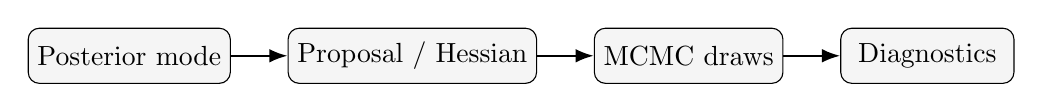
\begin{tikzpicture}[node distance=.72cm,>=Latex,every node/.style={draw,rounded corners,align=center,minimum width=2.2cm,minimum height=.7cm,fill=gray!8}]
\node (m) {Posterior mode};\node[right=of m] (h) {Proposal / Hessian};\node[right=of h] (s) {MCMC draws};\node[right=of s] (d) {Diagnostics};\draw[->,thick] (m)--(h);\draw[->,thick] (h)--(s);\draw[->,thick] (s)--(d);\end{tikzpicture}
\vfill The sampler approximates posterior expectations with draws, not a single point estimate.\end{frame}
\begin{frame}{MCMC diagnostics answer concrete questions}\begin{itemize}\item \key{Mixing:} do chains explore the posterior efficiently?\item \key{Convergence:} do independent chains give compatible summaries?\item \key{Effective sample size:} how much independent information remains after autocorrelation?\item \key{Prior--posterior comparison:} did the data move beliefs?\end{itemize}\end{frame}
\section{Dynare implementation}
\begin{frame}[fragile]{Estimation block: communicate assumptions}\small\begin{verbatim}
estimated_params;
  rho, beta_pdf, 0.80, 0.10;
  stderr e, inv_gamma_pdf, 0.01, 2;
end;
estimation(datafile=mydata, mode_compute=6,
           mh_replic=20000, mh_nblocks=2);
\end{verbatim}
\vfill\key{Read the code as a research protocol:} observables, priors, sample, algorithm and output choices must be explicit.
\end{frame}
\begin{frame}{A defensible empirical workflow}\begin{enumerate}\item Download and document data; transform it to model units.\item Verify the deterministic steady state and stochastic solution.\item Inspect prior predictive implications and estimate.\item Diagnose convergence and compare prior/posterior distributions.\item Interpret impulse responses and uncertainty economically.\end{enumerate}\end{frame}
\section{Course synthesis}
\begin{frame}{From theory to credible inference}\centering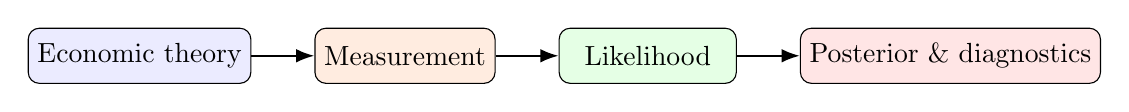
\begin{tikzpicture}[node distance=.8cm,>=Latex,every node/.style={draw,rounded corners,align=center,minimum width=2.25cm,minimum height=.7cm}]
\node[fill=blue!8] (a) {Economic theory};\node[fill=orange!12,right=of a] (b) {Measurement};\node[fill=green!10,right=of b] (c) {Likelihood};\node[fill=red!10,right=of c] (d) {Posterior \& diagnostics};\draw[->,thick] (a)--(b);\draw[->,thick] (b)--(c);\draw[->,thick] (c)--(d);\end{tikzpicture}
\vfill A good report makes every link in this chain inspectable and reproducible.\end{frame}
\begin{frame}{Assessment reminder}\begin{itemize}\item Choose one published model and write the report in English.\item Submit a LaTeX-produced PDF and complete reproducible code.\item Explain data, transformations, estimates and diagnostics.\item Do not include caches or unnecessary outputs.\end{itemize}\vfill\centering\Large\key{Submission deadline: 15 January 2027}\end{frame}
\end{document}
